\section{Introduction}
\label{sec:introduction}
Well, well, well. You want me to talk about namespaces... I have already done
great work in this field~\cite{sevilla:sc15-mantle, sevilla:sc15-malacology}.

% What is PLFS
PLFS~\cite{bent_plfs_2009} solved the checkpoint problem by mapping logical
files to physical files on the underlying file system. The solution targets N-1
strided checkpoints, where many processes write small IOs to offsets in the
same logical file. The key insight of PLFS is that general purpose file systems
perform well for applications that use N-N checkpoints and that the N-1 strided
checkpoint style can be transformed with a thin interposition layer. To map
offsets in the logical file to physical files each process maintains an index
of \{logical offset, physical offset, length, physical block id\}. 


\begin{figure}
  \centering
  \begin{subfigure}[b]{0.25\textwidth}
    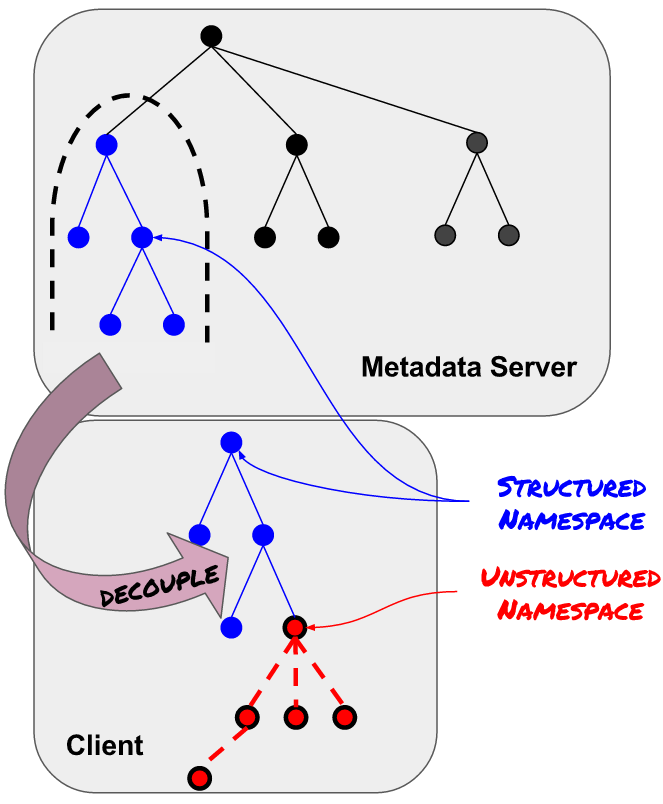
\includegraphics[width=\textwidth]{figures/intro.png}
   \label{fig:intro}
  \end{subfigure}
  ~ 
  \begin{subfigure}[b]{0.3\textwidth}
    \begin{tabular}{ r | l }
      Type         & Overhead       \\\hline\\
      Structured   & 1 RPC          \\
      Namespace    & O(1)           \\\\\hdashline\\
      Unstructured & 1 RPC + Replay \\
      Namespace    & O(1)           \\\\\hdashline\\
      Traditional  & \(n\) RPCs     \\
      Namespace    & O(\(n\))       \\
    \end{tabular}
    \\\\\\ % I am a hack
   \label{table:intro}
  \end{subfigure}
  \caption{Clients decouple the file system subtrees and interact with their
  private copiese locally for high performance. They can specify the structure of
  the metadata they intend to create (structured namespace) or they can create
  ad-hoc metadata (unstructured namespace), which is merged later.}
\end{figure}
%    \caption{Traditional namespaces require at least 1 RPC per metadata
%    operation. Structured namespaces only need the initial RPC so clients/servers
%    understand (and can construct) the namespace.  Unstructured namespaces cannot
%    be parallelized and must replay metadata one by one onto the global namespace}
 
% What is the problem?
The problem is that the underyling file system cannot keep up with the metadata
load imposed by PLFS. PLFS creates an index entry for every write, which
results in large per-processes tables ~\cite{grider:pc17-diddlings}. This makes
reading or scanning a logical file slow because PLFS must construct a global
index by reading each process's local index. This process incurrs a
\texttt{readdir} and, if the file is open by another process, an additional
\texttt{stat()} because metadata cannot be cached in the
container~\cite{bent_plfs_2009}.

% What is our solution
We propose XXX, a file system that uses the Cudele API, to succinctly express
metadata structure. Clients dictate the structure and patterns of the metadata
they intend to create for their workload to the underlying storage system. They
can also merge new metadata (that they did not explicitly state up front) into
the global namespace.  The benefits of the this approach are:

\begin{itemize}

  \item metadata compaction: describing the structure of the resulting
  namespace and inodes lets XXX enjoy the performance advantages
  of~\cite{he:hpdc13-plfs-patterns}

  \item reducing RPCs: if the client and server both understand the final
  structure of the file system metadata, there is no need to communicate; this
  results in higher throughput at the cost of increased latency for read operations

\end{itemize}

The idea uses concepts from decoupled namespaces~\cite{zheng:pdsw2014-batchfs,
zheng:pdsw2015-deltafs} and patterned IO~\cite{he:hpdc13-plfs-patterns} to
build a scalable global namespace. Less work is done on the metadata servers
and clients pick up some of the metadata load.  This approach is similar to
predicate push down in databases, where structure is described using XML or
JSON and pushed as predicates to the lower storage
layers~\cite{shel:pc17-pushdown}. It is our hope the XXX will also be able to
change the representation or structure of the file system metadata according to
the file type or workload.

We have the following contributions:

\begin{itemize}

  \item a prototype implementation, XXX, that leverages metadata
  compaction and reduces RPC amplification to improve performance

  \item structured and unstructured namespaces, a paradigm that helps
  applications optimize performance by giving the storage system information.

\end{itemize}


Caching can reduce RPC amplification but for
consitency writes (e.g., file creates) require at least one RPC. 
